\documentclass{article}[12pt]

\addtolength{\oddsidemargin}{-.75in}%
\addtolength{\evensidemargin}{-.75in}%
\addtolength{\textwidth}{1.5in}%
\addtolength{\textheight}{1.3in}%
\addtolength{\topmargin}{-.8in}%
\addtolength{\marginparpush}{-.75in}%
% \setlength\parindent{0pt}
% \setlength{\bibsep}{0pt plus 0.3ex}

\usepackage[authoryear]{natbib}
\usepackage{graphicx}
\usepackage{algorithm,algorithmic}

\title{Variational approximations for zero-inflated Semiparametric Regression models}
\author{Mark Greenaway, John T. Ormerod}

% include.tex
\newcommand{\Bernoulli}[1]{\text{Bernoulli} \left( #1 \right)}
\newcommand{\mydigamma}[1]{\psi \left( #1 \right)}
%\newcommand{\diag}[1]{\text{diag}\left( #1 \right)}
\newcommand{\tr}[1]{\text{tr}\left( #1 \right)}
\newcommand{\Poisson}[1]{\text{Poisson} \left( #1 \right)}
\def \half {\frac{1}{2}}
\def \R {\mathbb{R}}
\def \vbeta {\vec{\beta}}
\def \vy {\vec{y}}
\def \vmu {\vec{\mu}}
\def \vmuqbeta {\vmu_{q(\vbeta)}}
\def \vmubeta {\vmu_{\vbeta}}
\def \Sigmaqbeta {\Sigma_{q(\vbeta)}}
\def \Sigmabeta {\Sigma_{\vbeta}}
\def \va {\vec{a}}
\def \vtheta {\vec{\theta}}
\def \mX {\vec{X}}

\def\ds{{\displaystyle}}

\def\diag{{\mbox{diag}}}


\usepackage{latexsym,amssymb,amsmath,amsfonts}
%\usepackage{tabularx}
\usepackage{theorem}
\usepackage{verbatim,array,multicol,palatino}
\usepackage{graphicx}
\usepackage{graphics}
\usepackage{fancyhdr}
\usepackage{algorithm,algorithmic}
\usepackage{url}
%\usepackage[all]{xy}



\def\approxdist{\stackrel{{\tiny \mbox{approx.}}}{\sim}}
\def\smhalf{\textstyle{\frac{1}{2}}}
\def\vxnew{\vx_{\mbox{{\tiny new}}}}
\def\bib{\vskip12pt\par\noindent\hangindent=1 true cm\hangafter=1}
\def\jump{\vskip3mm\noindent}
\def\etal{{\em et al.}}
\def\etahat{{\widehat\eta}}
\def\thick#1{\hbox{\rlap{$#1$}\kern0.25pt\rlap{$#1$}\kern0.25pt$#1$}}
\def\smbbeta{{\thick{\scriptstyle{\beta}}}}
\def\smbtheta{{\thick{\scriptstyle{\theta}}}}
\def\smbu{{\thick{\scriptstyle{\rm u}}}}
\def\smbzero{{\thick{\scriptstyle{0}}}}
\def\boxit#1{\begin{center}\fbox{#1}\end{center}}
\def\lboxit#1{\vbox{\hrule\hbox{\vrule\kern6pt
      \vbox{\kern6pt#1\kern6pt}\kern6pt\vrule}\hrule}}
\def\thickboxit#1{\vbox{{\hrule height 1mm}\hbox{{\vrule width 1mm}\kern6pt
          \vbox{\kern6pt#1\kern6pt}\kern6pt{\vrule width 1mm}}
               {\hrule height 1mm}}}


%\sloppy
%\usepackage{geometry}
%\geometry{verbose,a4paper,tmargin=20mm,bmargin=20mm,lmargin=40mm,rmargin=20mm}


%%%%%%%%%%%%%%%%%%%%%%%%%%%%%%%%%%%%%%%%%%%%%%%%%%%%%%%%%%%%%%%%%%%%%%%%%%%%%%%%
%
% Some convenience definitions
%
% \bf      -> vector
% \sf      -> matrix
% \mathcal -> sets or statistical
% \mathbb  -> fields or statistical
%
%%%%%%%%%%%%%%%%%%%%%%%%%%%%%%%%%%%%%%%%%%%%%%%%%%%%%%%%%%%%%%%%%%%%%%%%%%%%%%%%

% Sets or statistical values
\def\sI{{\mathcal I}}                            % Current Index set
\def\sJ{{\mathcal J}}                            % Select Index set
\def\sL{{\mathcal L}}                            % Likelihood
\def\sl{{\ell}}                                  % Log-likelihood
\def\sN{{\mathcal N}}                            
\def\sS{{\mathcal S}}                            
\def\sP{{\mathcal P}}                            
\def\sQ{{\mathcal Q}}                            
\def\sB{{\mathcal B}}                            
\def\sD{{\mathcal D}}                            
\def\sT{{\mathcal T}}
\def\sE{{\mathcal E}}                            
\def\sF{{\mathcal F}}                            
\def\sC{{\mathcal C}}                            
\def\sO{{\mathcal O}}                            
\def\sH{{\mathcal H}} 
\def\sR{{\mathcal R}}                            
\def\sJ{{\mathcal J}}                            
\def\sCP{{\mathcal CP}}                            
\def\sX{{\mathcal X}}                            
\def\sA{{\mathcal A}} 
\def\sZ{{\mathcal Z}}                            
\def\sM{{\mathcal M}}                            
\def\sK{{\mathcal K}}     
\def\sG{{\mathcal G}}                         
\def\sY{{\mathcal Y}}                         
\def\sU{{\mathcal U}}  


\def\sIG{{\mathcal IG}}                            


\def\cD{{\sf D}}
\def\cH{{\sf H}}
\def\cI{{\sf I}}

% Vectors
\def\vectorfontone{\bf}
\def\vectorfonttwo{\boldsymbol}
\def\va{{\vectorfontone a}}                      %
\def\vb{{\vectorfontone b}}                      %
\def\vc{{\vectorfontone c}}                      %
\def\vd{{\vectorfontone d}}                      %
\def\ve{{\vectorfontone e}}                      %
\def\vf{{\vectorfontone f}}                      %
\def\vg{{\vectorfontone g}}                      %
\def\vh{{\vectorfontone h}}                      %
\def\vi{{\vectorfontone i}}                      %
\def\vj{{\vectorfontone j}}                      %
\def\vk{{\vectorfontone k}}                      %
\def\vl{{\vectorfontone l}}                      %
\def\vm{{\vectorfontone m}}                      % number of basis functions
\def\vn{{\vectorfontone n}}                      % number of training samples
\def\vo{{\vectorfontone o}}                      %
\def\vp{{\vectorfontone p}}                      % number of unpenalized coefficients
\def\vq{{\vectorfontone q}}                      % number of penalized coefficients
\def\vr{{\vectorfontone r}}                      %
\def\vs{{\vectorfontone s}}                      %
\def\vt{{\vectorfontone t}}                      %
\def\vu{{\vectorfontone u}}                      % Penalized coefficients
\def\vv{{\vectorfontone v}}                      %
\def\vw{{\vectorfontone w}}                      %
\def\vx{{\vectorfontone x}}                      % Covariates/Predictors
\def\vy{{\vectorfontone y}}                      % Targets/Labels
\def\vz{{\vectorfontone z}}                      %

\def\vone{{\vectorfontone 1}}
\def\vzero{{\vectorfontone 0}}

\def\valpha{{\vectorfonttwo \alpha}}             %
\def\vbeta{{\vectorfonttwo \beta}}               % Unpenalized coefficients
\def\vgamma{{\vectorfonttwo \gamma}}             %
\def\vdelta{{\vectorfonttwo \delta}}             %
\def\vepsilon{{\vectorfonttwo \epsilon}}         %
\def\vvarepsilon{{\vectorfonttwo \varepsilon}}   % Vector of errors
\def\vzeta{{\vectorfonttwo \zeta}}               %
\def\veta{{\vectorfonttwo \eta}}                 % Vector of natural parameters
\def\vtheta{{\vectorfonttwo \theta}}             % Vector of combined coefficients
\def\vvartheta{{\vectorfonttwo \vartheta}}       %
\def\viota{{\vectorfonttwo \iota}}               %
\def\vkappa{{\vectorfonttwo \kappa}}             %
\def\vlambda{{\vectorfonttwo \lambda}}           % Vector of smoothing parameters
\def\vmu{{\vectorfonttwo \mu}}                   % Vector of means
\def\vnu{{\vectorfonttwo \nu}}                   %
\def\vxi{{\vectorfonttwo \xi}}                   %
\def\vpi{{\vectorfonttwo \pi}}                   %
\def\vvarpi{{\vectorfonttwo \varpi}}             %
\def\vrho{{\vectorfonttwo \rho}}                 %
\def\vvarrho{{\vectorfonttwo \varrho}}           %
\def\vsigma{{\vectorfonttwo \sigma}}             %
\def\vvarsigma{{\vectorfonttwo \varsigma}}       %
\def\vtau{{\vectorfonttwo \tau}}                 %
\def\vupsilon{{\vectorfonttwo \upsilon}}         %
\def\vphi{{\vectorfonttwo \phi}}                 %
\def\vvarphi{{\vectorfonttwo \varphi}}           %
\def\vchi{{\vectorfonttwo \chi}}                 %
\def\vpsi{{\vectorfonttwo \psi}}                 %
\def\vomega{{\vectorfonttwo \omega}}             %


% Matrices
%\def\matrixfontone{\sf}
%\def\matrixfonttwo{\sf}
\def\matrixfontone{\bf}
\def\matrixfonttwo{\boldsymbol}
\def\mA{{\matrixfontone A}}                      %
\def\mB{{\matrixfontone B}}                      %
\def\mC{{\matrixfontone C}}                      % Combined Design Matrix
\def\mD{{\matrixfontone D}}                      % Penalty Matrix for \vu_J
\def\mE{{\matrixfontone E}}                      %
\def\mF{{\matrixfontone F}}                      %
\def\mG{{\matrixfontone G}}                      % Penalty Matrix for \vu
\def\mH{{\matrixfontone H}}                      %
\def\mI{{\matrixfontone I}}                      % Identity Matrix
\def\mJ{{\matrixfontone J}}                      %
\def\mK{{\matrixfontone K}}                      %
\def\mL{{\matrixfontone L}}                      % Lower bound
\def\mM{{\matrixfontone M}}                      %
\def\mN{{\matrixfontone N}}                      %
\def\mO{{\matrixfontone O}}                      %
\def\mP{{\matrixfontone P}}                      %
\def\mQ{{\matrixfontone Q}}                      %
\def\mR{{\matrixfontone R}}                      %
\def\mS{{\matrixfontone S}}                      %
\def\mT{{\matrixfontone T}}                      %
\def\mU{{\matrixfontone U}}                      % Upper bound
\def\mV{{\matrixfontone V}}                      %
\def\mW{{\matrixfontone W}}                      % Variance Matrix i.e. diag(b'')
\def\mX{{\matrixfontone X}}                      % Unpenalized Design Matrix/Nullspace Matrix
\def\mY{{\matrixfontone Y}}                      %
\def\mZ{{\matrixfontone Z}}                      % Penalized Design Matrix/Kernel Space Matrix

\def\mGamma{{\matrixfonttwo \Gamma}}             %
\def\mDelta{{\matrixfonttwo \Delta}}             %
\def\mTheta{{\matrixfonttwo \Theta}}             %
\def\mLambda{{\matrixfonttwo \Lambda}}           % Penalty Matrix for \vnu
\def\mXi{{\matrixfonttwo \Xi}}                   %
\def\mPi{{\matrixfonttwo \Pi}}                   %
\def\mSigma{{\matrixfonttwo \Sigma}}             %
\def\mUpsilon{{\matrixfonttwo \Upsilon}}         %
\def\mPhi{{\matrixfonttwo \Phi}}                 %
\def\mOmega{{\matrixfonttwo \Omega}}             %
\def\mPsi{{\matrixfonttwo \Psi}}                 %

\def\mone{{\matrixfontone 1}}
\def\mzero{{\matrixfontone 0}}

% Fields or Statistical
\def\bE{{\mathbb E}}                             % Expectation
\def\bP{{\mathbb P}}                             % Probability
\def\bR{{\mathbb R}}                             % Reals
\def\bI{{\mathbb I}}                             % Reals
\def\bV{{\mathbb V}}                             % Reals

\def\vX{{\vectorfontone X}}                      % Targets/Labels
\def\vY{{\vectorfontone Y}}                      % Targets/Labels
\def\vZ{{\vectorfontone Z}}                      %

% Other
\def\etal{{\em et al.}}
\def\ds{\displaystyle}
\def\d{\partial}
\def\diag{\text{diag}}
%\def\span{\text{span}}
\def\blockdiag{\text{blockdiag}}
\def\tr{\text{tr}}
\def\RSS{\text{RSS}}
\def\df{\text{df}}
\def\GCV{\text{GCV}}
\def\AIC{\text{AIC}}
\def\MLC{\text{MLC}}
\def\mAIC{\text{mAIC}}
\def\cAIC{\text{cAIC}}
\def\rank{\text{rank}}
\def\MASE{\text{MASE}}
\def\SMSE{\text{SASE}}
\def\sign{\text{sign}}
\def\card{\text{card}}
\def\notexp{\text{notexp}}
\def\ASE{\text{ASE}}
\def\ML{\text{ML}}
\def\nullity{\text{nullity}}

\def\logexpit{\text{logexpit}}
\def\logit{\mbox{logit}}
\def\dg{\mbox{dg}}

\def\Bern{\mbox{Bernoulli}}
\def\sBernoulli{\mbox{Bernoulli}}
\def\sGamma{\mbox{Gamma}}
\def\sInvN{\mbox{Inv}\sN}
\def\sNegBin{\sN\sB}

\def\dGamma{\mbox{Gamma}}
\def\dInvGam{\mbox{Inv}\Gamma}

\def\Cov{\mbox{Cov}}
\def\Mgf{\mbox{Mgf}}

\def\mis{{mis}} 
\def\obs{{obs}}

\def\argmax{\operatornamewithlimits{\text{argmax}}}
\def\argmin{\operatornamewithlimits{\text{argmin}}}
\def\argsup{\operatornamewithlimits{\text{argsup}}}
\def\arginf{\operatornamewithlimits{\text{arginf}}}


\def\minimize{\operatornamewithlimits{\text{minimize}}}
\def\maximize{\operatornamewithlimits{\text{maximize}}}
\def\suchthat{\text{such that}}


\def\relstack#1#2{\mathop{#1}\limits_{#2}}
\def\sfrac#1#2{{\textstyle{\frac{#1}{#2}}}}


\def\comment#1{
\vspace{0.5cm}
\noindent \begin{tabular}{|p{14cm}|}  
\hline #1 \\ 
\hline 
\end{tabular}
\vspace{0.5cm}
}


\def\mytext#1{\begin{tabular}{p{13cm}}#1\end{tabular}}
\def\mytextB#1{\begin{tabular}{p{7.5cm}}#1\end{tabular}}
\def\mytextC#1{\begin{tabular}{p{12cm}}#1\end{tabular}}

\def\jump{\vskip3mm\noindent}

\def\KL{\text{KL}}
\def\N{\text{N}}
\def\Var{\text{Var}}

\def \E {\mathbb{E}}
\def \BigO {\text{O}}
\def \IG {\text{IG}}
\def \Beta {\text{Beta}}



\begin{document}

\maketitle

Abstract: A Variational Bayes approach using Gaussian Variational Approximation to zero-inflated Poisson
regression models using the latent variable representation from \cite{Ghosh20061360} is presented. We
demonstrate on simulated and real datasets that our approach is flexible enough to handle random effects and
smoothing splines while remaining computationally efficient.

Keywords: Approximate Bayesian inference ; mixed model ; Markov chain Monte Carlo ; Stan ; 
					penalized splines .

\section{Introduction}
\label{sec:introduction}

Count data with a large number of zero counts arises in many areas of application, such as data arising from
physical activity studies, insurance claims, hospital visits or defects in manufacturing processes. These
models have been used for many applications, including defects in manufacturing in \cite{lambert1992},
horticulture in \cite{BIOM:BIOM1030} and \cite{Hall2000}, length of stay data from hospital admissions in
\cite{BIMJ:BIMJ200390024}, psychology in \cite{JOFP:rethink}, pharmaceutical studies in \cite{Min01042005},
traffic accidents on roadways in \cite{Shankar1997829} and longitudinal studies in
\cite{LeeWangScottYauMcLachlan2006}.

The strength of the approach derives from modelling the zero and non-zero count data seperately as a mixture
of distributions for the zero and non-zero components, allowing analysis of both the proportion of zeroes in
the data set and the conditions for the transition from zero to non-zero. When combined with a multivariate
mixed model regression framework, an extremely rich class of models can be fit allowing a broad range of
applications to be addressed. Often the transition from zero to non-zero has a direct interpretation in the
area of application, and is interesting in its' own right. In the example application presented in this paper,
the zero component represents an apartment completely free of roaches, while the non-zero component represents
an apartment where roaches have been able to live and reproduce, possibly in spite of pest control treatment
aimed at preventing them from doing so.

In this paper, we build upon the earlier work on Bayesian zero-inflated models of \cite{Ghosh20061360} and
\cite{VatsaWilson2014}. While simple forms of these models are easy to fit with standard maximum likelihood
techniques, more general models incorporating random effects, splines and missing data typically have no
closed form solutions and hence present a greater computational challenge to fit.

Fitting these models is typically done with Monte Carlo Markov Chain techniques, but these can be slow and
prone to convergence problems. We build upon a latent variable representation of these models to allow a
tractable Variational Bayes approximation to be derived. This allows us to fit close approximations to these
models using a deterministic algorithm which converges much more quickly.

We allow a flexible regression modelling approach by using a Gaussian Variational Approximation as defined in
\cite{ormerod09} on the regression parameters to allow a non-conjugate Gaussian prior to be used, making the
resulting Gaussian posterior of the regression parameters easy to interpret. We adopt a Mean Field Variational
Bayes (VB) approach on the other parameters in the model to derive the rest of the approximation.

The focus of this paper is on developing a method of fitting flexible ZIP regression models accurately, and
showing the advantages of our method to previously presented methods. In Section \ref{sec:methodology} we
briefly introduce Variational Bayes methodogy. In Section \ref{sec:model_and_data} we define our model and
provide a framework for our approach incorporating regression modelling and random effects. In Section
\ref{sec:algorithms} we present algorithms for fitting these models, along with a new parameterisation which
offers substantial advantages in accuracy, numerical stability and computational speed. In Section
\ref{sec:results} we perform numerical experiments on simulated data which show how our approach offers
computational advantages over existing approaches. In Section \ref{sec:application} we show an application of
our method to a multi-level longitudinal study of pest control in apartments. Finally, in Section
\ref{sec:discussion} we conclude with a discussion of the results. An appendix contains details of the
derivation of the variational lower bound for our model.

\section{Methodology}
\label{sec:methodology}

In this section we present a VB approach to a Bayesian zero-inflated Poisson model for count data with extra
zeroes. After introducing Bayesian zero-inflated models and VB methodology we derive the VB factorised
approximation to the full Bayesian model.

\subsection{Variational Bayesian inference}

Semiparametric mean field Variational Bayes is an approximate Bayesian inference method as detailed in
\cite{ormerod10} and \cite{RohdeWand2015}.

The approximation is fit by iteratively minimising the Kullback-Leibler divergence between the true posterior
and an approximating distribution. Thus the optimal approximation $q^*(\vtheta)$ is

$$
q^*(\vtheta) = \argmin_{\vxi \in \Xi} \text{KL} \{ {q(\vtheta|\vxi) || p(\vtheta|\vy)} \}.
$$

A common approach is to assume an approximation in a factorised form

$$q(\vtheta) = \Pi_{i=1}^M q(\theta_i).$$

The variational lower bound is maximised iteratively. On each iteration, the value of each parameter in the
model is calculated as the expectation of the full likelihood relative to the other parameters in the model,
which is referred to as the mean field update:

$$q_i^*(\theta_i) \propto \exp{\{ \bE_{-q(\theta_i)} \log p(\vy, \vtheta) \}}$$

This is done for each parameter in the model in turn until the variational lower bound's increase is
negligible and convergence is achieved.

This approach works well for classes of models where all of the parameters are conjugate. For more general
classes of models, mean field updates are not analytically tractable and general gradient-based optimisation
methods must be used, as for the Gaussian Variational Approximation (see \cite{ormerod09}) used in this paper.
These methods are generally difficult to apply in practice, as the problems can involve the optimisation of
many parameters over high-dimensional, constrained spaces whose constraints cannot be simply expressed.

\section{The zero-inflated Poisson regression model}
\label{sec:model_and_data}

Variational approximations are well-suited to accelerating the fit of Bayesian zero-inflated models to data.
Typically zero-inflated models arise in applications where we wish to build multivariate regression models. To
be able to construct multivariate models with as much generality as possible, we specify the full model as a
General Design Bayesian Generalized Linear Mixed Model, as in \citep{zhao06}. This allows us to incorporate
within-subject correlation, measurement error, missing data and smoothing splines (as in \cite{Wand2008}) in
our models.

% Idea: We can use an approximation of the from q(\beta, \u, \Sigma) q(\rho) \Product q(r_i)
% and use GVA on q(\beta, \u, \Sigma) and mean field updates on \rho and r_i

\subsection{Model and data}

The $j$th predictor/response pair for the $i$th group is denoted by $(\vx_{ij}, \vy_{ij}), 1 \leq j \leq n_i,
1 \leq i \leq m$, where the $\vx_{ij}$ are unrestricted, while the $\vy_{ij}$ are nonnegative integers.

For each $1 \leq i \leq m$, define the $n_i \times 1$ vectors $\vy_{ij} = [\vy_{i 1}, \ldots, \vy_{i
n_i}]^\top$ and $\vone_i = [1, \ldots, 1]^\top$, where the first of these vectors is the response. It is
reasonable to assume that the vectors $\vy_1, \ldots, \vy_m$ are independent of each other.

Let $\mR = \diag{(\vr)}$, $\mC = [\mX, \mZ]$ and $\vnu = [\vbeta^\top, \vu^\top]^\top$. Consider the model

$$
\begin{array}{rl}
\log{p(\vy|\vr, \vbeta, \vu)} &= \vy^\top \mR (\mC\vnu) - \vr^\top \exp{(\mC\vnu)} - \vone^\top \log{\Gamma{(\vy + \vone)}}, \\
\mbox{ and }
r_i &\sim \text{Bernoulli}(\rho), 1 \leq i \leq n \\
\end{array}
$$

with priors

$$ 
\begin{array}{rl}
\log{p(\mSigma_{\vu \vu})} &= \text{Inverse Wishart}(\mPsi, v),\\
p(\rho) &\propto 1 \\
\mbox{ and } \vnu|\sigma_\vu^2 &\sim \mbox{N}(\vzero, \sigma_\vu^2 \mI)\\
\end{array}
$$

where $\mX$ is $n \times p$, $\mZ$ is $n \times mb$ and $\mSigma_{\vu \vu}$ and $\mPsi$ are $b \times b$.

\subsection{Approximation}
Let $\vr_0 = \{ r_i : y_i = 0 \}$.
We assume an approximation of the form
$$
q(\vr_0, \vnu, \sigma_{\vu}^2, \rho) = q(\vnu) q(\mSigma_{\vu \vu}) q(\rho) q(\vr_0) \\
$$

where 
$q(\sigma_{\vu}^2) = \mbox{Inverse Wishart}\left(\mPsi + \sum_{i=1}^m \vmu_i \vmu_i^\top + \mLambda_{\vu_i \vu_i}, v + m + 
p\right)$ \mbox{and } $q(r_i) = \Bernoulli{(p_i)}$

with
$$
p_i = \expit\left[ \psi{(\alpha_{q(\rho)})} - \psi{(\beta_{q(\rho)})} - \exp{(c_i^\top\vmu + \half c_i^\top \mLambda c_i)} \right]
$$

\text{when} $\vy_i = 0$.

%$\propto \exp{\left \{-r_i \bE_{-r_i} [\exp{(c_i^\top\vnu)}] + r_i [\psi(\alpha_\rho) - \psi(\beta_\rho)] \right \} }.\\$

The optimal approximation for $\vr$ is
$$
\begin{array}{rl}
q(\vr) &\propto \exp \left [ \bE_{-q(\vr)}\vy^\top\mR(\mC\vmu) - \vr^\top\exp{(\mC\vnu)}-\half \vnu^\top \mSigma_{\vu \vu} \vnu \right ] \\ [1ex]
	&= \exp{ \left\{ \vy^\top\mR\mC \vmu - \vr^\top \exp{[\mC \vmu + \half \text{diag}(\mC \mLambda \mC^\top)]} - \half \vmu^\top \mD \vmu - \half \text{tr}(\mLambda \mD ) \right\} }
\end{array}
$$

where $\mD = \left[ (\mPsi + \sum_{i=1}^m \vmu_i \vmu_i^\top + \mLambda_{\vu_i\vu_i}) / (v - p - 1) \right]^{-1}$. 

This is close in form to a Poisson regression model. Poisson regression models with normal priors have no
closed form for their mean field updates due to non- conjugacy, but can be fit using Gaussian Variational
Approximation, as in \citep{ormerod09}. The model can be fit using Algorithm \ref{alg:algorithm_one} below.

\begin{algorithm}
\caption[Algorithm 1]{Iterative scheme for obtaining the parameters in the
optimal densities $q^*(\vmu, \mLambda)$, $q^*(\mSigma_{\vu \vu})$ and $q^*(\rho)$}
\label{alg:algorithm_one}
\begin{algorithmic}
\REQUIRE{$\alpha_{q(\rho)} \leftarrow \alpha_\rho + \vone^\top\vp, p_{q(\mSigma_{\vu \vu})} \leftarrow p + 1$} \\[1ex]
\WHILE{the increase in $\log{\underline{p}}(\vy;q)$ is significant}
% \vmu, \mLambda
\STATE Optimise $\vmu$ and $\mLambda$ using $\vy, \mC, \vp$ and $\mSigma_{\vu \vu}$ \\[1ex]
% \vp
\STATE $\beta_{q(\rho)} \leftarrow \beta_\rho + n - \vone^\top\vp$ \\[1ex]
\STATE $\eta \leftarrow -\exp \left [ \mC \vmu + \half \diag{(\mC\mLambda\mC^\top)} \right ] + \psi{(\alpha_{q{(\rho)}})} - \psi{(\beta_{q{(\rho)}})}$ \\[1ex]
\STATE $\vp_{q(\vr_0)} \leftarrow \expit{(\eta)}$ \\[1ex]
% \mSigma_{\vu \vu}
\STATE $\mPsi_{q(\mSigma_{\vu \vu})} \leftarrow \Psi + \sum_{i=1}^m \vmu_i \vmu_i^\top + \mLambda_{{\vu}_i}$ \\[1ex]
\STATE $\mSigma_{\vu\vu} \leftarrow [\mPsi_{q(\mSigma_{\vu \vu})}/(v - d - 1)]^{-1}$
\ENDWHILE
\end{algorithmic}
\end{algorithm}

\section{Numerical optimisation strategies}
\label{sec:algorithms}

In this section, we compare the accuracy, stability and speed of a number of algorithms for fitting the
Gaussian component of our model.

\subsection{Laplace-Variational Approximation}

Laplace's method of approximation uses the second order Taylor expansion of the full log likelihood around the
mode to find a Gaussian approximation to the full posterior. This can then be optimised using Newton-Raphson
style iterations. The algorithm is very quick to execute, but the resulting approximate posterior
distributions are not as accurate as those produced by the other algorithms considered in this article.

% NR
% Detail the function and its derivatives

Taylor expanding the full log likelihood once around the mode yields the following function
\begin{align*}
\log \underline{p}(\vmu, \mLambda; \vy) = \vy^\top\mP\mC\vmu - \vp^\top\exp \left (\mC \vmu \right ) - \half \vmu^\top \mSigma^{-1} \vmu.
\end{align*}

This can be optimised using a Newton-Raphson style algorithm where
\begin{align*}
\frac{\partial \log p(\vmu, \mLambda; \vy)}{\partial \vmu} &\approx \mP \mC (\vy - \exp{(\mC \vmu)}) - \mSigma^{-1} \vmu \text{ and} \\
\frac{\partial \log p(\vmu, \mLambda; \vy)}{\partial \mLambda} &\approx - \mC^\top \text{diag}(\vp e^{(\mC \vmu)}) \mC - \mSigma^{-1}.
\end{align*}

The steps of the algorithm are shown in Algorithm \ref{alg:laplace_alg}.

\begin{algorithm}
\caption{Laplace scheme for optimising $\log \underline{p}(\vmu, \mLambda; \vy)$}
\label{alg:laplace_alg}
\begin{algorithmic}
% Fit \vmu, \mLambda using Laplace approximation
\WHILE{the increase in $\log \underline{p}(\vmu, \mLambda; \vy)$ is significant}
% \vmu, \mLambda
\STATE $\mLambda \leftarrow \left [\mP \mC^\top \text{diag}(\exp{(\mC \vmu)}) \mC + \mSigma^{-1} \right ]^{-1}$ \\ [1ex] 
\STATE $\vmu \leftarrow \vmu + \mLambda \left [ \frac{\partial \log p(\vmu, \mLambda; \vy)}{\partial \vmu} \right ]$ \\ [1ex]
\ENDWHILE
\end{algorithmic}
\end{algorithm}

\subsection{Optimising the GVA lower bound}

% Detail techniques used for fitting models.

Assuming $q(\vnu) \sim N(\vmu, \mLambda)$, the Gaussian variational lower bound in Algorithm
\ref{alg:algorithm_one} can be optimised using a variety of algorithms. The variational lower bound is not
necessarily unimodal, leading to potential difficulty in optimising to the global maximum. However, for fixed
$\vp$ and $\mSigma$, the variational lower bound is log-concave, and so standard optimisation methods such as
L-BFGS-B as described in, for example, \cite{Liu1989}, work well. This led to an extremely accurate
approximation of the true posterior at the expense of some additional computational effort.

\subsubsection{GVA}

The first variant of the Gaussian Variational Approximation algorithm optimises the Gaussian variational lower
bound of the log likelihood with respect to $\vmu$ and the Cholesky decomposition $\mR$ of $\mLambda$, that
is, $\mLambda = \mR \mR^\top$. This algorithm trades the computational complexity of numerically evaluating an
integral for greatly increased accuracy in the approximating posterior distribution. The resulting function is
below and can be optimised with L-BFGS-B.
% Detail the function and its derivatives
\begin{align*}
\log \underline{p}(\vmu, \mLambda; \vy) &= \quad \vy^\top\mP \mC \vmu - \vp^\top \exp[\mC \vmu + \half \text{diag}(\mC \mLambda \mC^\top)] - \half \vmu^\top \mSigma^{-1} \vmu - \half \tr{(\mSigma^{-1} \mLambda)} + \log{|\mR|} \\
&\quad - \tfrac{p}{2} \log{(2 \pi)} + \half \log{|\mSigma^{-1}|} + \tfrac{p}{2} \log{(2 \pi)} + \tfrac{p}{2} \\
\end{align*}

using the derivatives
\begin{align*}
\frac{\partial \log \underline{p}(\vmu, \mLambda; \vy)}{\partial \vmu} &= \mP \mC (\vy - \mC^\top \exp(\mC \vmu + \half \text{diag}{(\mC \mLambda \mC^\top)})) - \mSigma^{-1} \vmu \text{ and}\\
\frac{\partial \log \underline{p}(\vmu, \mLambda; \vy)}{\partial \mLambda} &= \left [\mLambda^{-1} - \mP \mC^\top \exp(\mC \vmu + \half \text{diag}(\mC \mLambda \mC^\top)) \mP \mC) - \mSigma^{-1} \right ] \mR.
\end{align*}

\subsubsection{GVA, new parameterisation}

The second variant of the Gaussian Variational Approximation algorithm is similiar to the first, but instead
of optimising the Gaussian variational lower bound with respect to $\vmu$ and the Cholesky factor $\mR$ of
$\mLambda$, we instead optimise the Cholesky factor of the inverse of $\mLambda$ i.e. $\mLambda = (\mR
\mR^\top)^{-1}$. This algorithm is henceforth referred to as GVA NP.

This new choice of parameterisation allows us to calculate $\exp(\mC \vmu + \half \text{diag}(\mC \mLambda
\mC^\top))$ and its derivatives by solving the linear system $\mR \va = \mC_{i}, i=1, \ldots, n$ for $\va$ and
then calculating $\va^\top\va$ rather than calculating $\text{diag}(\mC \mLambda \mC^\top)$ directly.

By interchanging the fixed and random effects in $\mC = [\mX \mZ]$ to $\mC = [\mZ \mX]$, and re- ordering the
dimensions of $\vmu, \mLambda$ and $\mSigma$ in the same manner, the independence between the blocks relating
to the random effects in $\mZ$ induce sparsity in the Cholesky factor $\mR$ of $\mLambda^{-1}$. Thus the
Gaussian $q(\vnu) \sim N(\vmu, \mLambda)$ can be optimised over a space of dimension $\half p (p + 1) + pq +
\half q (q + 1)$ rather than dimension $\half (p + mq) (p + mq + 1)$ as in the dense parameterisation. This
leads to subtantial performance gains when m is large, as is typically the case in problems of practical
importance such as longitudinal or clinical trials or the application presented in Section
\ref{sec:application}.

The Gaussian variational lower bound in this parameterisation is
\begin{align*}
\log \underline{p}(\vmu, \mLambda; \vy) &= \quad \vy\mP\mC \vmu - \vp^\top \exp(\mC \vmu + \half \text{diag}(\mC \mLambda \mC^\top)) - \half \vmu^\top \mSigma^{-1} \vmu - \half \tr{(\mSigma^{-1} \mLambda)} \\
&\quad- \tfrac{p}{2} \log{(2 \pi)} + \half \log{|\mSigma^{-1}|} + \tfrac{p}{2} \log{(2 \pi)} + \tfrac{p}{2} - \log{|\mR|}
\end{align*}

The derivative with respect to $\vmu$ is the same as that in the GVA algorithm, but as the parameterisation of
$\mLambda$ has changed, the  derivative with respect to $\mLambda$ becomes
\begin{align*}
\frac{\partial \log \underline{p}(\vmu, \mLambda; \vy)}{\partial \mLambda}
&= \hphantom{-}(\mLambda^{-1} + \mH)(-\mLambda \mR \mLambda) \\
&= -(\mI + \mH\mLambda)\mR\mLambda \\
&= - (\mR\mLambda + \mH\mLambda\mR\mLambda)
\end{align*} 

where $\mH = (\mP \mC)^\top \text{diag}(\exp(\mC \vmu + \half \mC \mLambda \mC^\top)) \mP \mC - \mSigma^{-1}$.


\subsubsection{GVA fixed point}

% Fixed point update of \mLambda

This variant of the algorithm uses Newton-Raphson-like fixed point updates on the Gaussian variational lower
bound. This algorithm is fast, but unstable. The steps are presented in Algorithm \ref{alg:algorithm_nr} where
\begin{align*}
\frac{\partial \log \underline{p}(\vmu, \mLambda; \vy)}{\partial \vmu} &= \quad \mC^\top\vp \left [\vy - \mC\exp(\mC \vmu + \half \text{diag}(\mC \mLambda \mC^\top)) \right ] - \mSigma^{-1} \vmu \text{ and}\\
\frac{\partial \log \underline{p}(\vmu, \mLambda; \vy)}{\partial \mLambda} &= -\mC^\top \text{diag}(\vp^\top \exp(\mC \vmu +\half \text{diag}(\mC \mLambda \mC^\top))) - \mSigma^{-1}.
\end{align*}

\begin{algorithm}
\caption[Algorithm GVA NR]{Iterative scheme for obtaining optimal $\vmu$ and $\mLambda$
given $\vy$, $\mC$ and $\vp$}
\label{alg:algorithm_nr}
\begin{algorithmic}
% Fit \vmu, \mLambda using Laplace approximation
\WHILE{the increase in $\log{\underline{p}}(\vmu, \mLambda; \vy)$ is significant}
% \vmu, \mLambda
\STATE $\mLambda \leftarrow \left [ \mP^\top \mC^\top \exp(\mC \vmu + \half \text{diag}(\mC \mLambda \mC^\top)) \mC \mP \right ]^{-1}$ \\ [1ex]
\STATE $\vmu \leftarrow \vmu + \mLambda \left [ \frac{\partial \log \underline{p}(\vmu, \mLambda; \vy)}{\partial \vmu} \right ]$
\ENDWHILE
\end{algorithmic}
\end{algorithm}

% Splines

\section{Numerical results}
\label{sec:results}

The accuracy of each model fitting algorithm presented in Section \ref{sec:algorithms} was assessed by
comparing the approximating distribution of each parameter with the posterior distribution of Monte Carlo
Markov Chain samples of that parameter. 1 million Monte Carlo Markov Chain samples were generated using Stan.
The accuracy of examples of random intercept, random slope and spline models were evaluated using this method.

\subsection{Simulated data}

For each of these simulations, the model is as presented in Section \ref{sec:methodology}.

Several common application scenarios were simulated and their accuracy evaluated. A random intercept model was
simulated with $\vbeta = (2, 1)^\top$, $\rho = 0.5$, $m = 20$, $n_i = 10$ and $b = 1$. The results are
presented in Table \ref{tab:accuracy_int}. A random slope model was simulated with $\vbeta = (2, 1)^\top$,
$\rho = 0.5$, $m = 20$, $n_i = 10$ and $b = 2$. The results are presented in Table \ref{tab:accuracy_slope}.
Spline model was fit to a data set generated from the function $3 + 3 \sin{(\pi x)}$ on the interval $[-1,
1]$. The resulting model fits are presented in Figure \ref{fig:spline}.

% The stability of the algorithms was confirmed by running them on 10,000 different data sets that were randomly
% generated after having initialised the random number generator with different seeds.

Median accuracy of the algorithms was assessed by running them on 100 randomly generated data sets. The
results are presented in Figure \ref{fig:median_accuracy_intercept} and Figure
\ref{fig:median_accuracy_slope}.

% Figure: Median accuracy graph intercept
\begin{figure}
\caption{Median accuracy of random intercept}
\label{fig:median_accuracy_intercept}
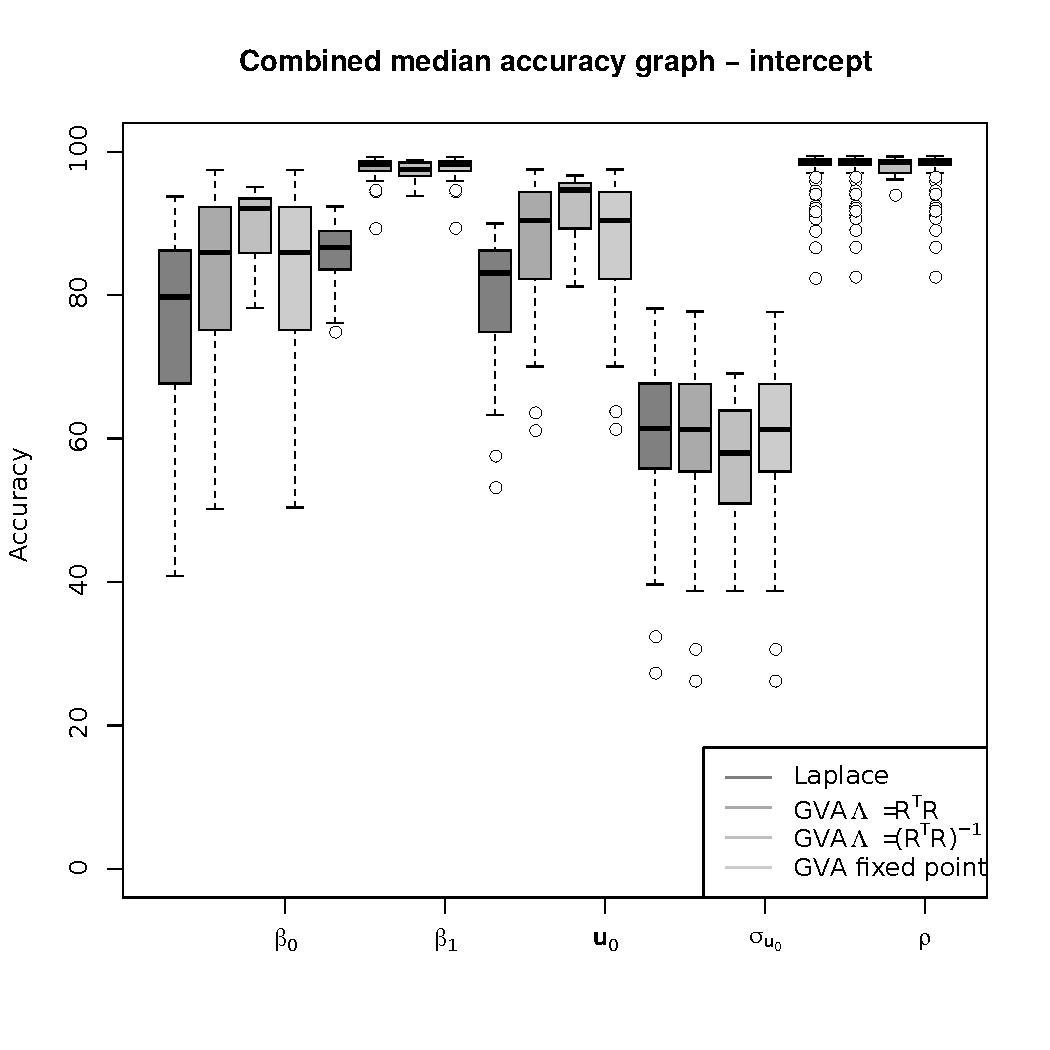
\includegraphics[width=100mm, height=100mm]{code/results/median_accuracy_combined_intercept.pdf}
\end{figure}

% Figure: Median accuracy graph slope
\begin{figure}
\caption{Median accuracy of slope}
\label{fig:median_accuracy_slope}
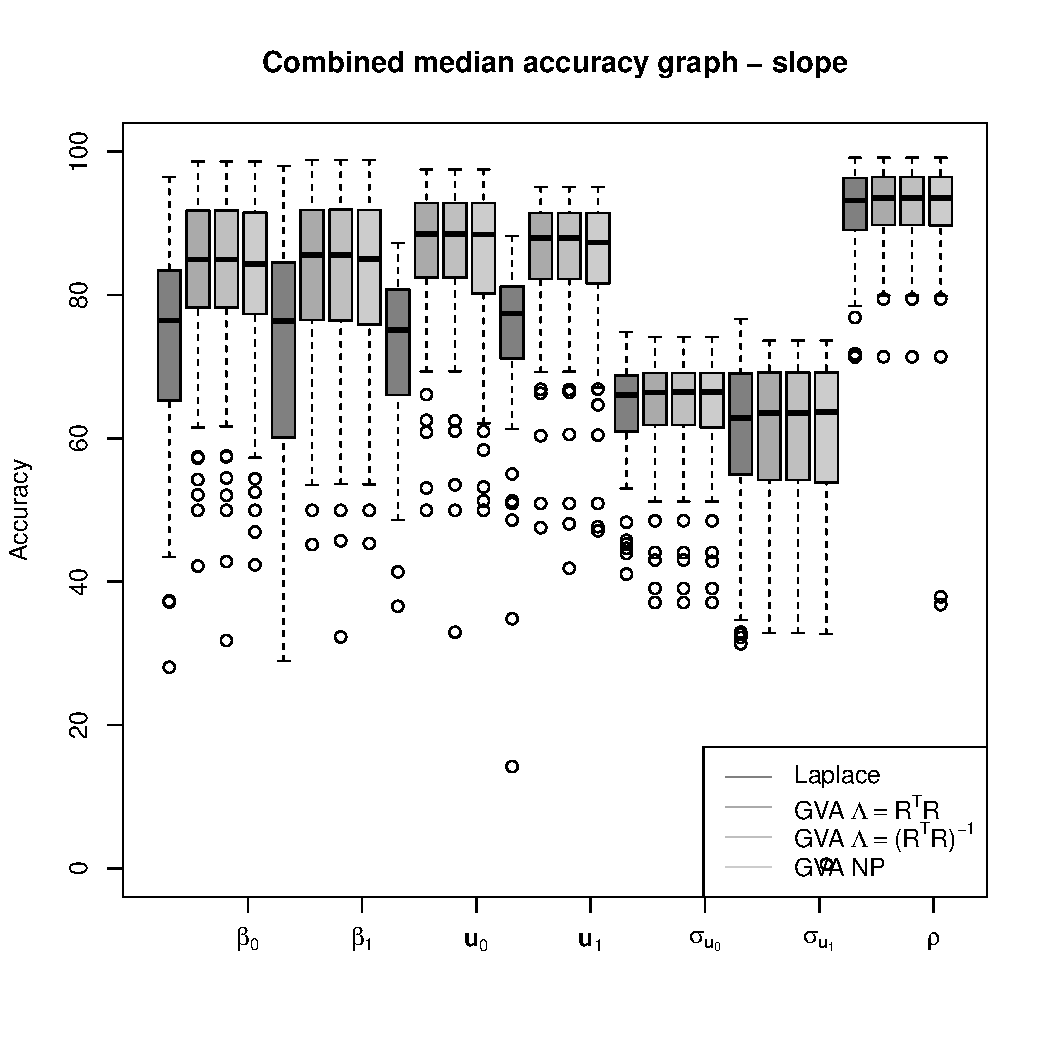
\includegraphics[width=120mm, height=120mm]{code/results/median_accuracy_combined_slope.pdf}
\end{figure}

% Table of accuracy results - intercept model
\begin{table}
\caption{Table of accuracy - Random intercept model}
\label{tab:accuracy_int}
\begin{tabular}{|l|rrrr|}
\hline
& Laplace's Method & GVA $(\mLambda = \mR \mR^\top)$ & GVA NP $(\mLambda = (\mR \mR^\top)^{-1})$ & GVA FP\\
\hline
$\vbeta_1$ & $83\%$ & $91\%$ & $91\%$ & $91\%$ \\ 
$\vbeta_2$ & $77\%$ & $99\%$ & $99\%$ & $99\%$ \\ 
Mean of $\vu$ & $81\%$ & $95\%$ & $95\%$ & $95\%$ \\
$\sigma^2_{\vu_1}$ & $63.0\%$ & $63.4\%$ & $63.4\%$ & $63.4\%$ \\ 
$\rho$ & $98\%$ & $97\%$ & $97\%$ & $97\%$ \\ 
\hline
\end{tabular}
\end{table}

\begin{table}
\caption{Table of accuracy - Random slope model}
\label{tab:accuracy_slope}
\begin{tabular}{|l|rrrr|}
\hline
& Laplace's Method & GVA $(\mLambda = \mR \mR^\top)$ & GVA $(\mLambda = (\mR \mR^\top)^{-1})$ & GVA FP\\
\hline
$\vbeta_1$   &66\%&88\%&89\%&88\%\\
$\vbeta_2$   &69\%&88\%&90\%&88\%\\
Mean of $\vu$    &72\%&91\%&91\%&91\%\\
$\sigma^2_{\vu_1}$ &69.6\%&71.5\%&71.5\%&71.5\%\\
$\sigma^2_{\vu_2}$ &65.9\%&67.6\%&67.6\%&67.6\%\\
$\rho$ &91\%&90\%&90\%&90\%\\
\hline
\end{tabular}
\end{table}

% \begin{table}
% \caption{Table of accuracy - Splines}
% \label{tab:accuracy_spline}
% \begin{tabular}{|l|l|}
% \hline
% Approximation & Accuracy \\
% \hline
% Laplace's Method & 0.969 \\
% GVA & 0.969 \\
% GVA NP & 0.969 \\
% GVA NR & 0.969 \\
% \hline
% \end{tabular}
% \end{table}

\begin{figure}
\label{fig:spline}
\caption{Comparison of VB and MCMC spline fits with the true function}
\includegraphics[width=100mm, height=100mm]{code/results/accuracy_plots_spline_GVA2.pdf}
\end{figure}

% Graphs - exactly what sort of graphs do we need?
% Median accuracy
% Increase in lower bound
% MCMC posterior, with approximating posterior for at least one or two of the
% key parameters, such as, say, vbeta[2]

\subsection{Stability results}

The numerical stability of each fitting algorithm in Section \ref{sec:algorithms} was assessed by initialising
each algorithm from a range of different starting points. Errors due to numerical instability and the fitted
$\vmu$ were recorded for each starting point.

A data set of 100 individuals in ten groups (m=10) was generated from a model with a fixed intercept
and slope, and a random intercept. $\vmu$ was initialised from a grid of points on the interval
$[-4.5, 5]$ for intercept and slope. The error counts are presented in Table
\ref{tab:stability_results}.

\begin{table}
\caption{Count of numerical errors for each algorithm during stability tests}
\label{tab:stability_results}
\begin{tabular}{|l|r|}
\hline
Algorithm & Error count \\
\hline
Laplace's algorithm & 12 \\
GVA & 1,771 \\
GVA NP & 537 \\
GVA FP & 992 \\
\hline
\end{tabular}
\end{table}

\section{Application}
\label{sec:application}

% TODO: You need to describe the data set and the model.

The model fitting was applied to the cockroach data set from \cite{Gelman2007} taken from a study on the
effect of integrated pest management in controlling cockroach levels in urban apartments. The data set
contains data on 160 treatment and 104 control apartments, along with the response $y_i$ in each apartment of
the number of cockroaches caught in a set of traps. The apartments had the traps deployed for different
numbers of days, referred to as trap days, which was handled by using a log offset \cite{Agresti2002}. The
predictors in the data set included the pre-treatment roach level, a treatment indicator, the time of the
observation and an indicator for whether the apartment is in a senior building restricted to the elderly.

The GVA NP algorithm was used to fit a random intercept model to the Roaches data set provided by Andrew
Gelman. The fitted co-efficients and accuracy results are presented in Table \ref{tab:application_roaches}.

%       lci  uci
% 1  3.179 3.157 3.201
% 2 -0.046 -0.053 -0.039
% 3 -0.420 -0.434 -0.406
% 1 -0.976 -1.015 -0.936
% 2 -0.309 -0.323 -0.295
% 3 -0.947 -0.963 -0.930
% 4 -2.129 -2.384 -1.874
% 5 -3.230 -3.490 -2.970
% 6 -3.099 -3.404 -2.794
% 7 -1.290 -1.326 -1.255
% 8 -0.956 -0.991 -0.921
% 9 -2.404 -2.600 -2.209
% 10 -1.076 -1.123 -1.029
% 11 -1.079 -1.107 -1.052
% 12 -1.681 -1.737 -1.624

%> round(cbind(fit1$vmu, lci, uci), 3)
% fit1$a_rho
% [1] 377.2375
% > fit1$b_rho
% [1] 152.7625

\begin{table}
\caption{Table of results - Roaches}
\label{tab:application_roaches}
\begin{tabular}{|l|rrrr|}
\hline
Covariate & Posterior Mean & Lower 95\% CI & Upper 95\% CI & Accuracy \\
\hline
Intercept & 3.18 & 3.16 & 3.20 & 90\% \\
Time & $-$0.05 & $-$0.05 & $-$0.04 & 97\% \\
Time:Treatment & $-$0.43 & $-$0.43 & $-$0.41 & 93\% \\
Random intercept & $-$1.60 & $-$1.71 & $-$1.49 & 90\% \\
$\sigma^2_{\vu_1}$ & 0.58 & 0.57 & 0.57 & 57\% \\
$\rho$ & 0.71 & 0.67 & 0.75 & 88\% \\
\hline
\end{tabular}
\end{table}

\begin{figure}
	\caption{Accuracy graphs for roach model}
	\label{fig:accuracy_roach}
	\centering
	% \includepdf[width=75mm,height=75mm,pages={1,2,3,16},nup=2x2]{code/results/accuracy_plots_application_GVA2.pdf}
	\begin{tabular}{@{}c@{\hspace{.5cm}}c@{}}
		\includegraphics[page=1,width=.45\textwidth]{code/results/accuracy_plots_application_GVA2.pdf} & 
		\includegraphics[page=2,width=.45\textwidth]{code/results/accuracy_plots_application_GVA2.pdf} \\[.5cm]
		\includegraphics[page=3,width=.45\textwidth]{code/results/accuracy_plots_application_GVA2.pdf} &
		\includegraphics[page=16,width=.45\textwidth]{code/results/accuracy_plots_application_GVA2.pdf} \\[.5cm]
	\end{tabular}
\end{figure}

To assess the speed of each approach, a test case was constructed of a random slope model with $m=50$ groups,
each containing $n_i = 100$ individuals. A model was then fit to this data set ten times using each algorithm,
and the results averaged. They are presented in Table \ref{tab:application_slope_speed}. It should be noted
that the speed of the GVA and GVA FP algorithms was impaired by their implementation in R using the
\texttt{optim()} function, which makes many function calls during its' execution. If the same algorithms were
re-implemented in another language with a vectorising compiler and modern well-implemented numerical linear
algebra libraries such as C++, the performance would be substantially improved.

\begin{table}
\caption{Table of results - Speed}
\label{tab:application_slope_speed}
\begin{tabular}{|l|rr|}
\hline
Algorithm & Mean (seconds) & Standard deviation (seconds) \\
\hline
Laplace's method & 18.79 s & 0.07 s \\
GVA & 76.18 s & 1.24 s \\
GVA NP & 27.55 s & 0.66 s \\
GVA FP & 4.83 s & 0.07 s \\
\hline
\end{tabular}
\end{table}

\section{Discussion}
\label{sec:discussion}
\begin{itemize}
\item Numerical issues
\item What worked well
\item What didn't
\end{itemize}

\newpage
\section{Appendix} 
% TODO: Mean field updates?
\subsection{Calculation of the Variational Lower bound}
% Where are the priors for \vbeta and \vu

The variational lower bound is equal to $\bE_q[\log{p(\vy, \vtheta)} - \log{q(\vtheta)}] = T_1 + T_2 + T_3$,
where

% This is the new T_1
$$
\begin{array}{rl}
T_1 &= \quad \bE_q[\log{p(\vy, \vnu)} - \log{q(\vnu)}] \\
&= \quad \vy \mP \mC \vmu - \vp^\top \exp{\left[ \mC \vmu + \half \text{diag} (\mC \mLambda \mC^\top) \right]} - \vone^\top\log \Gamma{(\vy + \vone)}\\
& \quad + \frac{p + m}{2} (1 + \log{2 \pi}) + \half \log{|\mLambda|}, \\
T_2 &= \quad \bE_q \left[ \log p(\mSigma_{\vu \vu}) - \log q(\mSigma_{\vu \vu}) \right] \\
&= \quad \bE_q \big[ v/2(\log |\Psi| - \log |\Psi + \vmu_\vu \vmu_\vu^\top + \mLambda_{\vu \vu}|) + \half \log 2 + \half \log|\mSigma_{\vu \vu}| + \log \Gamma_{p+1}(v/2) - \log \Gamma_{p}(v/2)\\
&\quad + \half \tr((\vmu_{\vu} \vmu_{\vu}^\top + \mLambda_{\vu \vu}) \mSigma_{\vu \vu}^{-1}) \big] \\
&= \quad v/2\big(\log |\Psi| - \log |\Psi + \vmu_\vu \vmu_\vu^\top + \mLambda_{\vu \vu}|\big) + \half \log 2 + \half \bE_q \log |\mSigma_{\vu \vu}| + \log \Gamma_{p+1}(v/2) - \log \Gamma_{p}(v/2) \\
&\quad + \half \tr\big(\mI_m + \Psi(\Psi+ \vmu_\vu \vmu_\vu^\top + \mLambda_{\vu \vu})^{-1}/(v + p + 2)\big) \\
T_3 &= - \vp^\top \log \vp - (\vone - \vp)^\top \log (\vone - \vp) - \log \Beta (\alpha_\rho, \beta_\rho) + \log \Beta (\alpha_q, \beta_q)
\end{array}
$$

with $\bE_q \big[ \log |\mSigma_{\vu \vu}| \big] = m \log 2 + \log \left | \Psi + \vmu_\vu \vmu_\vu^\top + \mLambda_{\vu \vu} \right | + \sum_{i=1}^m \Psi \left ( \frac{v - i + 1}{2} \right )$

\subsection{Numerical stability of fitting algorithms with respect to starting point}

% TODO: Generate images using local_solutions.R and place here

\bibliographystyle{elsarticle-harv}
\bibliography{Chapter_1_zero_inflated_models}

\end{document}
